\chapter{Considerações Finais}

\section{Trabalhos Futuros}

O trabalho atual pode permitir que um time melhor
seja criado modificando-se os parâmetros da função
objetivo ou adicionando novos custos à função objetivo.
Assim, o modelo de competição apresentado na
figura~\ref{fig:mod_comp} pode ser utilizado.

\begin{figure}[H]
  \centering
  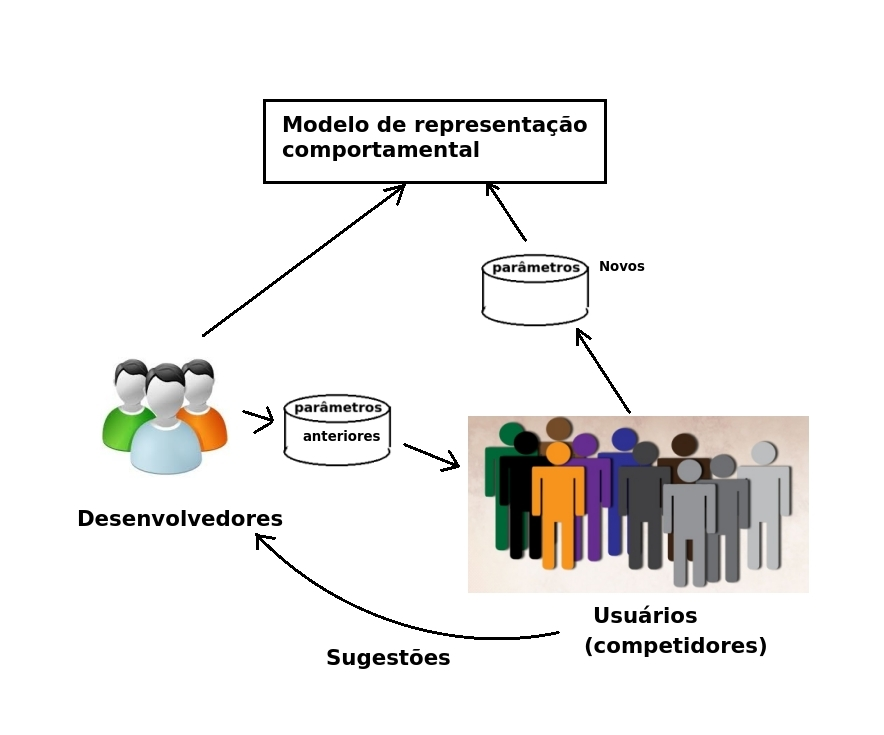
\includegraphics[width=0.8\linewidth]{mod_comp}
  \caption{Modelo de Competição para melhorar
           o time}\label{fig:mod_comp}
\end{figure}

Dessa forma, através do fornecimento dos parâmetros
vencedores da competição anterior, tem-se um avanço
no desempenho do time.

Outra forma de se melhorar o time é utilizar uma
maneria automática para realizar as partidas e
avaliar o desempenho do time nessa partida. Isso
permitiria que algorítimos de otimização também
fossem utilizados para melhorar os parâmetros.
Uma das dificuldades desta abordagem é a necessidade
de se alterar o simulador para reposicionar a bola
ou os robôs durante a partida.
 
%\section{Dificuldades}
%
%minimax --> otimização --> função objetivo
%com muitas característica --> problemas
%--> talvez um minimax com uma função mais
%    simples (possibilidade de se incorporar
%    poda alpha e beta



